% MAT670 -- Lecture 3 (18.4.2016) -- transcribed from MAT670_3, pp. 32--48 of the handwritten notes
\chapter[Lecture 3: Blichfeldt gauges, Kabatjanskii--Levenshtein]{Lecture 3: Blichfeldt gauges and the Kabatjanskii--Levenshtein bound}
\label{L3:ch}

\noindent\emph{Lecture of 18 April 2016.}\orig{Notes pp.~32--48.}
Last time we proved the Fejes T\'oth inequality for point configurations on the sphere and
Blichfeldt's sphere packing bound. Today we make some remarks on both, look at the landscape of
known bounds for the packing density, prove the Kabatjanskii--Levenshtein-type bound via a Blichfeldt
gauge, and then extend the notion of a Blichfeldt gauge from balls to general convex bodies.

\added{Throughout, ``a packing of unit balls'' means a family of balls of radius $1$ in $\R^n$ with
pairwise disjoint interiors, i.e.\ with centers at mutual distance at least $2$.}

%======================================================================
\section{Some remarks}
\label{L3:sec:remarks}

\subsection*{Where is the Fejes T\'oth inequality sharp?}

Recall the Fejes T\'oth inequality: \added{if $n\ge 3$ points are placed on the unit sphere $\Sph^2\subset\R^3$,
then the minimal angular distance $d$ between two of them satisfies}
\begin{equation}\label{L3:eq:FT}
  d \;\le\; \arccos\!\left(\frac{\cot^2\omega-1}{2}\right),
  \qquad \omega=\frac{n}{n-2}\cdot\frac{\pi}{6}.
\end{equation}
\fixed{Notes have $\cot(\omega)$; the square is needed (check $n=12$).}%
The right-hand side is the angular edge length of the equilateral spherical triangle with area
$\frac{4\pi}{2n-4}$ on the unit sphere. \added{(A triangulation of the sphere with $n$ vertices has $2n-4$
triangular faces, so this is the area of a face when the $4\pi$ of total area is split evenly.)}

So the bound should be sharp exactly when the points are the vertices of an equilateral deltahedron
\added{(a polytope all of whose faces are congruent equilateral triangles) inscribed in the sphere}, i.e.\ for
\[
  n = 3,\ 4,\ 6,\ 12,
\]
and perhaps asymptotically as $n\to\infty$.
\begin{addedblock}
Check: $n=3$ gives $\omega=\pi/2$, $d\le\arccos(-\tfrac12)=120^\circ$ (an equilateral triangle on a great circle, the degenerate case);
$n=4$ gives $\cot^2\omega=\tfrac13$, $d\le\arccos(-\tfrac13)\approx109.47^\circ$ (regular tetrahedron);
$n=6$ gives $\omega=\pi/4$, $d\le 90^\circ$ (regular octahedron);
$n=12$ gives $\omega=\pi/5$, $d\le\arccos(1/\sqrt5)\approx 63.43^\circ$ (regular icosahedron).
Equality requires a triangulation by congruent equilateral triangles, so these are the only cases of equality;
as $n\to\infty$ the bound is asymptotically sharp.
\end{addedblock}
\orig{$n=3$ underlined in the notes.}

There are other proofs of the Fejes T\'oth inequality, but they are longer.

%======================================================================
\section{Aside: Blichfeldt's gauge revisited}
\label{L3:sec:aside}
\orig{Numbered ``3.2 aside''. Crossed out above: ``Again, there exists e.g.\ a trivial Blichfeldt gauge for $C$, given by $\chi_C$.''}

We saw last time that
\begin{equation}\label{L3:eq:f0}
  f_0(x)=\begin{cases} 1-\tfrac12\abs{x}^2, & \abs{x}\le\sqrt2,\\[2pt] 0, & \abs{x}>\sqrt2,\end{cases}
\end{equation}
is a Blichfeldt gauge for $\Ball^n$: \added{for every packing of unit balls with centers $c_1,c_2,\dots$,
$\sum_i f_0(x-c_i)\le 1$ for all $x\in\R^n$, and consequently the packing density satisfies
$\dens\le \vol(\Ball^n)/\int_{\R^n}f_0$.}
It is non-trivial for our purposes, that is,
\[
  \int_{\R^n} f_0(x)\,dV \;>\; \int_{\R^n}\chi_{\Ball^n}\,dV=\vol(\Ball^n)
  \qquad\text{(at least for } n>2).
\]
Indeed,
\begin{equation}\label{L3:eq:intf0}
  \int_{\R^n} f_0(x)\,dV=\frac{2^{1+\frac n2}}{n+2}\,\vol(\Ball^n).
\end{equation}
\begin{addedblock}
Proof: in polar coordinates, $dV = n\vol(\Ball^n)\,t^{n-1}\,dt\,d\sigma$ (with $\sigma$ the normalized surface measure), so
\[
  \int f_0 = n\vol(\Ball^n)\int_0^{\sqrt2}\Bigl(1-\frac{t^2}{2}\Bigr)t^{n-1}\,dt
  = \vol(\Ball^n)\Bigl(2^{n/2}-\frac{n}{2(n+2)}2^{(n+2)/2}\Bigr)
  = \frac{2\cdot 2^{n/2}}{n+2}\vol(\Ball^n).
\]
Hence $\int f_0>\vol(\Ball^n)$ iff $2^{1+n/2}>n+2$, which holds exactly for $n\ge3$; for $n=2$ there is equality and for
$n=1$ the gauge is worse than $\chi_{\Ball^1}$.
\end{addedblock}

\subsection*{From the gauge to the density bound}
Consider a packing $P$ of unit balls and a large cube $\mathrm{Box}(t)$ of side length $t$.
\begin{addedblock}
Split the balls meeting $\mathrm{Box}(t)$ into the \emph{inner} ones, whose centers lie in the concentric cube of side
$t-2\sqrt2$, and the \emph{boundary} ones. The support of $f_0(\cdot-c_i)$ for an inner center lies in $\mathrm{Box}(t)$, so
integrating $\sum_i f_0(x-c_i)\le 1$ over $\mathrm{Box}(t)$ gives
$N_{\mathrm{in}}\int f_0\le t^n$. The boundary centers lie in a shell of bounded width around $\partial\,\mathrm{Box}(t)$,
so there are at most $C\,t^{n-1}$ of them (by a volume argument, $C$ depending only on $n$).
\end{addedblock}
Therefore, for all $t$,
\[
  \frac{\vol\bigl(P\cap \mathrm{Box}(t)\bigr)}{\vol\bigl(\mathrm{Box}(t)\bigr)}
  \;\le\; \frac{n+2}{2^{1+\frac n2}} \;+\; \frac{C\,t^{n-1}}{t^n},
\]
\fixed{Notes: main term times $(1+\frac{\sqrt2-2}{t})^n$ (Lecture~2: $2\sqrt2-2$); not needed here, tends to $1$.}%
and letting $t\to\infty$,
\begin{equation}\label{L3:eq:blichfeldt}
  \dens(\Ball^n)\;\le\;\limsup_{t\to\infty}\frac{\vol(P\cap\mathrm{Box}(t))}{\vol(\mathrm{Box}(t))}\;\le\;\frac{n+2}{2^{1+\frac n2}}.
\end{equation}

\begin{remark}
We could equally well use
\[
  \dens=\limsup_{t\to\infty}\frac{\vol\bigcup\{\,\Ball\in P:\ \Ball\subseteq\mathrm{Box}(t)\,\}}{\vol\bigl(\mathrm{Box}(t)\bigr)},
\]
\added{counting only the balls entirely inside the box; since the balls meeting $\partial\,\mathrm{Box}(t)$ have total volume
$O(t^{n-1})$, this gives the same limit.}
\end{remark}

%======================================================================
\section{What does this look like?}
\label{L3:sec:landscape}
\orig{Section number overwritten: ``3.3'' / ``4''.}

The bound \eqref{L3:eq:blichfeldt} coming from $f_0$ gives the following density bounds
\added{(two-digit values as in the notes)}:
\begin{center}
\begin{tabular}{c|cccccccccc}
\toprule
$n$ & 1 & 2 & 3 & 4 & 5 & 6 & 7 & 8 & 9 & 10\\
\midrule
$\dfrac{n+2}{2^{1+n/2}}$ & 1.06 & 1 & .88 & .75 & .61 & .5 & .39 & .31 & .24 & .19\\
\bottomrule
\end{tabular}
\end{center}
\added{For comparison, the true optimal densities are $1$, $\pi/\sqrt{12}\approx .9069$, $\pi/\sqrt{18}\approx .7405$ in dimensions $1,2,3$,
and $\pi^4/384\approx .2537$ in dimension $8$.}

\subsection*{Asymptotic bounds}
\begin{center}
\begin{tabular}{p{0.44\textwidth}|p{0.44\textwidth}}
\textbf{Lower bounds} & \textbf{Upper bounds}\\
\midrule
$\dfrac{1}{2^n}$ \ (saturation) & $\dfrac{n+2}{2^{\frac n2+1}}$ \ (Blichfeldt)\\[10pt]
\quad$\vdots$ & \quad$\vdots$\\[4pt]
Ball (1992): $\dfrac{2n}{2^n}$ & $2^{-0.599n}$ \ (Kabatjanskii--Levenshtein)\\[10pt]
Vance, $n\equiv 0 \bmod 4$: $\dfrac{6}{e}\cdot\dfrac{n}{2^n}$ & \quad (Cohn, Elkies, Kumar, \dots)\\[10pt]
Venkatesh (sparse) \added{(2013)}: $\dfrac{1}{2}\cdot\dfrac{n\log\log n}{2^n}$ \ (!!!) & \\
\end{tabular}
\end{center}
\fixed{Notes: $e^{-\gamma}/2$; Venkatesh proves $\Delta_n\ge n\log\log n/2^{n+1}$, i.e.\ $1/2$.}%
\begin{addedblock}
Comments. (1) \emph{Saturation:} if a packing of unit balls is saturated (no further ball can be added), then the balls of
radius $2$ with the same centers cover $\R^n$, so $2^n\dens\ge 1$; saturated packings exist (e.g.\ by Zorn's lemma or a greedy
construction), hence $\dens(\Ball^n)\ge 2^{-n}$. (2) Ball (1992) proved $\dens\ge 2(n-1)\zeta(n)2^{-n}$ for lattice packings;
Vance (2011) proved $\dens\ge \frac{6n}{e\,2^n}$ for lattice packings when $4\mid n$; Venkatesh (\emph{A note on sphere packings in
high dimension}, IMRN 2013) proved $\dens\ge 65963\,n\,2^{-n}$ for all large $n$ and
$\dens\ge \frac12\,n\log\log n\,2^{-n}$ for infinitely many $n$ (the ``!!!'': the first improvement over linear growth of the
numerator). The $\log\log n$ comes from cyclotomic lattices: by Mertens' theorem $m/\varphi(m)$ can be as large as about
$e^{\gamma}\log\log m$. (3) \emph{Update after 2016:} Campos, Jenssen, Michelen and Sahasrabudhe (2023) proved
$\dens\ge(\frac12-o(1))\,n\log n\,2^{-n}$ for all $n$, and Klartag (2025) proved $\dens\ge c\,n^2 2^{-n}$ (even for lattice packings).
On the upper side, the exponent $0.599$ of Kabatjanskii--Levenshtein (1978) has only been improved by subexponential factors
(e.g.\ Cohn--Zhao 2014).
\end{addedblock}

\subsection*{Known good constructions}
There are known good constructions in low dimensions and special ones \added{(e.g.\ $D_4$, $E_8$, the Leech lattice $\Lambda_{24}$)}.
We need to talk about these at some point.\orig{Margin doodle (sad face) omitted.}

\subsection*{Exact results (upper bounds that are attained)}
\begin{itemize}
\item $d=1$: trivial.
\item $d=2$: we proved it. \added{Thue (1892, 1910); the first complete proof is due to L.~Fejes T\'oth (1940). The optimal lattice
packing was known to Lagrange and Gauss.}\unclear{Notes: ``(1892\dots ???) Thue''.}
\item $d=3$: Hales, twice, around 2000; a complicated geometric analysis. \added{Hales (with Ferguson), announced 1998, published in
Ann.\ of Math.\ 2005; the formal computer verification (Flyspeck project) was completed in 2014.}
\item $d=8$ and $d=24$: one month ago, via linear programming duality: one constructs a special (``magic'') auxiliary function.
\added{Viazovska (dimension 8, March 2016) and Cohn--Kumar--Miller--Radchenko--Viazovska (dimension 24, a week later);
both published in Ann.\ of Math.\ 2017. The LP bound itself is due to Cohn--Elkies (2003).}
\end{itemize}

\begin{remark}
Remember that the cubic lattice $\Z^n$ gives a packing of balls of radius $\frac12$ with density
\[
  \dens(\Z^n)=\vol\bigl(\tfrac12\Ball^n\bigr)=\frac{\pi^{n/2}}{2^n\,(\frac n2)!},
\]
\added{where $(\frac n2)!:=\Gamma(\frac n2+1)$. This decays superexponentially, much faster than the lower bound $2^{-n}$.}
\end{remark}

%======================================================================
\section{Kabatjanskii and Levenshtein}
\label{L3:sec:KL}

\begin{definition}\label{L3:def:M}
For $\varphi\in(0,\pi]$, let $M(d,\varphi)$ be the maximum number of points on $\Sph^{d-1}$ with pairwise
\added{angular} distance at least $\varphi$.
Equivalently, $M(d,\varphi)$ is the maximum number of points in $\R^d\setminus\{0\}$ such that the angle
\added{at the origin} spanned by any two of them is at least $\varphi$ \added{(project radially onto the sphere)}.
\end{definition}
\added{For example $M(d,\pi)=2$, and $M(d,\pi/3)=\kiss_d$ is the kissing number ($\kiss_2=6$, $\kiss_3=12$, $\kiss_4=24$, $\kiss_8=240$,
$\kiss_{24}=196560$).}

\begin{theorem}\label{L3:thm:KLgauge}
\added{In any dimension $d$}\orig{Notes: ``in high dimensions''.} and for $1<r<2$, the function
\[
  f_d(x)=\begin{cases} M\bigl(d,\arccos(1-\tfrac{2}{r^2})\bigr)^{-1}, & \abs{x}<r,\\[2pt] 0, & \abs{x}\ge r,\end{cases}
\]
is a Blichfeldt gauge for $\Ball^d$.
\end{theorem}

The key geometric fact is the following.

\begin{lemma}\label{L3:lem:angle}
Let $r<2$, let $x\in\R^d$ and let $y,z\in\R^d$ with $\abs{y-z}\ge 2$ and $\abs{x-y},\abs{x-z}\le r$. Then the angle $\theta$ at $x$
spanned by the segment $[y,z]$ satisfies $\cos\theta\le 1-\frac{2}{r^2}$, i.e.\ $\theta\ge\arccos(1-\frac2{r^2})$.
\end{lemma}

\begin{figure}[ht]
\centering
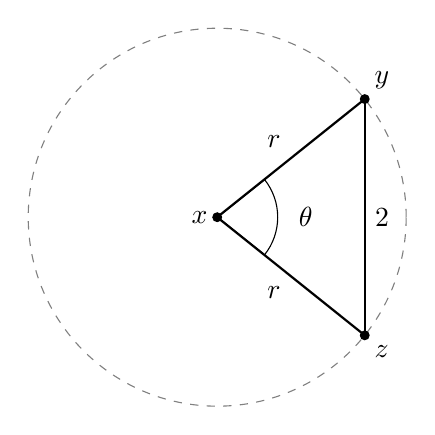
\begin{tikzpicture}[scale=1.5]
  \coordinate (X) at (0,0);
  \coordinate (Y) at (1.249,1.0);
  \coordinate (Z) at (1.249,-1.0);
  \draw[dashed,gray] (X) circle (1.6);
  \draw[thick] (X) -- (Y) node[midway,above left] {$r$};
  \draw[thick] (X) -- (Z) node[midway,below left] {$r$};
  \draw[thick] (Y) -- (Z) node[midway,right] {$2$};
  \draw (0.4,0.32) arc (38.66:-38.66:0.512);
  \node at (0.75,0) {$\theta$};
  \fill (X) circle (1.2pt) node[left] {$x$};
  \fill (Y) circle (1.2pt) node[above right] {$y$};
  \fill (Z) circle (1.2pt) node[below right] {$z$};
\end{tikzpicture}
\caption{The extremal case of Lemma~\ref{L3:lem:angle}: both centers at distance exactly $r$ from $x$ and at distance $2$ from each
other; then $\sin(\theta/2)=1/r$.}
\label{L3:fig:angle}
\end{figure}

\begin{proof}
First suppose both points are at distance exactly $r$ from $x$ (the worst case, see Figure~\ref{L3:fig:angle}).
Put $a=(y-x)/r$, $b=(z-x)/r$, unit vectors with $a\cdot b=\cos\theta$, and let $\ell=\abs{y-z}\ge2$. Then
\[
  \Bigl|\frac2r\Bigr|^2\le\Bigl|\frac{\ell}{r}\Bigr|^2=\abs{a-b}^2=2-2\,a\cdot b=2-2\cos\theta,
\]
so $\frac{4}{r^2}\le 2-2\cos\theta$, i.e.\ $\frac2{r^2}\le1-\cos\theta$, which is
\[
  \boxed{\cos\theta\le 1-\frac{2}{r^2}.}
\]
\begin{addedblock}
Why this is the worst case: in general, with $\alpha=\abs{x-y}$, $\beta=\abs{x-z}\in(0,r]$, the law of cosines gives
$\cos\theta=\frac{\alpha^2+\beta^2-\ell^2}{2\alpha\beta}\le h(\alpha,\beta):=\frac{\alpha^2+\beta^2-4}{2\alpha\beta}$, and
$\partial_\alpha h=\frac{\alpha^2-\beta^2+4}{2\alpha^2\beta}>0$ because $\beta\le r<2$. By symmetry $h$ is increasing in each variable,
so $h(\alpha,\beta)\le h(r,r)=1-\frac2{r^2}$. Equivalently, the apex angle of the isosceles triangle with legs $r$ and base $2$ is
$2\arcsin(1/r)$, and $\cos(2\arcsin\frac1r)=1-\frac2{r^2}$.
\end{addedblock}
\fixed{Side sketch says apex angle $2\arccos(1/r)$; it is $2\arcsin(1/r)$.}%
\end{proof}

\begin{proof}[Proof of Theorem~\ref{L3:thm:KLgauge}]
Take any packing of unit balls in $\R^d$ and $r<2$. For every $x\in\R^d$ there are at most $M\bigl(d,\arccos(1-2/r^2)\bigr)$ centers at
distance less than $r$ from $x$: by Lemma~\ref{L3:lem:angle}, the angle at $x$ spanned by any segment of length $\ge2$ whose ends are within
$r$ of $x$ is at least $\arccos(1-2/r^2)$, so the directions from $x$ to these centers form a configuration as in
Definition~\ref{L3:def:M}. \added{(If $x$ is itself a center, all other centers are at distance $\ge2>r$, and the count is $1$.)}
Hence $\sum_i f_d(x-c_i)\le 1$.
\end{proof}

\begin{corollary}\label{L3:cor:KL}
For $1\le r<2$,
\[
  \dens(\Ball^d)\le r^{-d}\,M\bigl(d,\arccos(1-\tfrac{2}{r^2})\bigr).
\]
Equivalently, substituting $r=1/\sin(\varphi/2)$,
\[
  \dens(\Ball^d)\le \sin\bigl(\tfrac\varphi2\bigr)^d\,M(d,\varphi),\qquad \frac\pi3<\varphi\le\pi.
\]
\end{corollary}
\begin{proof}
\added{$\int f_d=r^d\vol(\Ball^d)/M$, so $\dens\le\vol(\Ball^d)/\int f_d=r^{-d}M$. For the substitution: $1-\frac{2}{r^2}=1-2\sin^2\frac\varphi2=\cos\varphi$,
and $r\in[1,2)$ corresponds to $\varphi\in(\pi/3,\pi]$.}
\end{proof}
\added{Letting $r\to2$ recovers the simple bound $\dens(\Ball^d)\le \kiss_d\,2^{-d}$.}

For $d$ large, take $\varphi\approx63^\circ$; the Kabatjanskii--Levenshtein bound on spherical codes gives
\[
  \sin\bigl(\tfrac\varphi2\bigr)^d M(d,\varphi)\le 2^{-0.599d+o(d)},
\]
and hence
\[
  \dens(\Ball^d)\le 2^{-0.599d+o(d)}.
\]
\begin{addedblock}
More precisely, Kabatjanskii and Levenshtein (1978), using linear programming bounds for spherical codes, proved
$M(d,\varphi)\le 2^{d(c(\varphi)+o(1))}$ for $0<\varphi<\pi/2$, where with $s=\sin\varphi$,
\[
  c(\varphi)=\frac{1+s}{2s}\log_2\frac{1+s}{2s}-\frac{1-s}{2s}\log_2\frac{1-s}{2s}.
\]
The exponent $c(\varphi)+\log_2\sin(\varphi/2)$ is minimized at $\varphi^*\approx 62.9974^\circ$, where it equals $-0.5990\ldots$
(see Conway--Sloane, \emph{Sphere Packings, Lattices and Groups}, Ch.~1 and~9).
\end{addedblock}

%======================================================================
\section{Blichfeldt gauges for general bodies}
\label{L3:sec:general}
\orig{Section number overwritten, presumably 3.5.}

So we defined a Blichfeldt gauge for $\Ball^n$. Can we extend this? Abstractly:

\begin{definition}\label{L3:def:gauge}
Given a (convex) body $C$ in $\R^n$, a function $f:\R^n\to\R$ is a \emph{Blichfeldt gauge for $C$} if for any collection of
isometries $\{\varphi_i\}_{i=1}^\infty$ of $\R^n$ such that $\{\varphi_iC\}_{i=1}^\infty$ is a packing,
\[
  \sum_{i=1}^\infty f(\varphi_i^{-1}x)\le 1\qquad\forall x\in\R^n.
\]
\end{definition}
\added{As for balls, integrating over a large box shows that if $f$ is integrable and compactly supported, then every packing of
congruent copies of $C$ has density at most $\vol(C)/I(f)$, where $I(f):=\int_{\R^n}f$.}

\begin{remark}
One could add a non-negativity condition on $f$; what we really want is that the mass of $f$ is large: $I(f)\ge I(\chi_C)$.
\end{remark}
\begin{remark}
The index set could also be finite.
\end{remark}
\begin{remark}
The function $f$ could be much stranger than what we allow here.\unclear{Rest of the remark illegible: ``\dots accuracy first''?}
\end{remark}
\begin{exercise}[$\ast\ast\ast$]
Think about such functions distributionally.
\end{exercise}

There always exists a Blichfeldt gauge for $C$, e.g.\ $\chi_C$ \added{(the copies $\varphi_iC$ have disjoint interiors, so a point lies in
the interior of at most one of them; here one should take $\chi$ of the interior, or note that boundaries have measure zero)}.

\begin{lemma}\label{L3:lem:scaling}
If $f(x)$ is a Blichfeldt gauge for $C$, then $f(x/\lambda)$ is a Blichfeldt gauge for $\lambda C$, the $\lambda$-scaling of $C$.
\end{lemma}
\added{Indeed, a packing $\{\varphi_i(\lambda C)\}$ is the image under $x\mapsto\lambda x$ of the packing $\{\psi_iC\}$ with
$\psi_i(y)=\lambda^{-1}\varphi_i(\lambda y)$.}
For instance, $f_0$ (supported on the ball of radius $\sqrt2$) is a gauge for $\Ball^n$, and $f_0(x/\lambda)$ (supported on the ball of
radius $\lambda\sqrt2$) is a gauge for $\lambda\Ball^n$.\orig{Diagram of this scaling omitted.}

\begin{definition}\label{L3:def:inradius}
For a body $C$ define its \emph{inradius} $r(C)$ to be the radius of the largest sphere \added{(ball)} contained in $C$.
For $0\le\gamma\le r(C)$ define $C_\gamma$, the \emph{inner parallel body at depth $\gamma$}, to be the set of points
\[
  C_\gamma:=\{x\in C:\ x+\gamma\Ball^n\subseteq C\}.
\]
\end{definition}
\added{If $C$ is convex and compact, then $C_\gamma$ is convex, compact and non-empty for $\gamma\le r(C)$.}
We can define the straight-line distance from a point $x$ to a body $C$ by $d(x,C)$ \added{$=\min_{y\in C}\abs{x-y}$}.

\begin{figure}[ht]
\centering
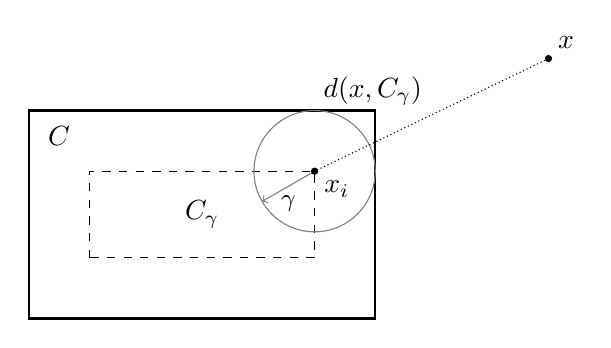
\begin{tikzpicture}[scale=1.1]
  \draw[thick] (0,0) rectangle (4,2.4);
  \draw[dashed] (0.7,0.7) rectangle (3.3,1.7);
  \node at (2,1.2) {$C_\gamma$};
  \node at (0.35,2.1) {$C$};
  \draw[gray] (3.3,1.7) circle (0.7);
  \draw[->,gray] (3.3,1.7) -- ++(-150:0.7) node[midway,below,black] {\small$\gamma$};
  \fill (3.3,1.7) circle (1.2pt) node[below right] {$x_i$};
  \fill (6,3) circle (1.2pt) node[above right] {$x$};
  \draw[densely dotted] (6,3) -- (3.3,1.7) node[midway,above left] {$d(x,C_\gamma)$};
\end{tikzpicture}
\caption{The inner parallel body $C_\gamma$ and the nearest point $x_i\in C_\gamma$ to $x$; the ball $x_i+\gamma\Ball^n$ lies in $C$.}
\label{L3:fig:parallel}
\end{figure}

\begin{theorem}\label{L3:thm:parallel}
Let $C$ be a convex body, $0<\gamma\le r(C)$, and let $f$ be a radial Blichfeldt gauge for $\Ball^n$, i.e.\ $f(x)=F(\abs x)$.
Define
\[
  g(x)=F\Bigl(\frac{d(x,C_\gamma)}{\gamma}\Bigr).
\]
Then $g$ is a Blichfeldt gauge for $C$.
\end{theorem}

This is fairly easy to see from a picture (Figure~\ref{L3:fig:parallel}).

\begin{proof}
We would like to show that
\[
  \sum_{i=1}^\infty g(\varphi_i^{-1}x)\le1\qquad\forall x\in\R^n,\ \text{for all packings }\{\varphi_iC\}_{i=1}^\infty \text{ of } C.
\]
Consider a point $x\in\R^n$ and, for each $i$, a point $x_i\in\varphi_iC_\gamma$ at distance $d(x,\varphi_iC_\gamma)$ from $x$
\added{(it exists since $C_\gamma$ is compact)}. Then $x_i+\gamma\Ball^n$ is contained in $\varphi_iC$
\added{(note $\varphi_iC_\gamma=(\varphi_iC)_\gamma$)}, and so $\{x_i+\gamma\Ball^n\}_i$ is a packing.
\orig{Parenthetical: ``since $C$ is convex, things are well defined''.}%
Since $F(\abs{y}/\gamma)$ is a Blichfeldt gauge for $\gamma\Ball^n$ (Lemma~\ref{L3:lem:scaling}), and $x$ is at distance
$\abs{x-x_i}=d(x,\varphi_iC_\gamma)$ from $x_i$, we get
\[
  \sum_i g(\varphi_i^{-1}x)=\sum_i F\Bigl(\frac{d(x,\varphi_iC_\gamma)}{\gamma}\Bigr)=\sum_i F\Bigl(\frac{\abs{x-x_i}}{\gamma}\Bigr)\le 1,
\]
\added{using $d(\varphi_i^{-1}x,C_\gamma)=d(x,\varphi_iC_\gamma)$ because $\varphi_i$ is an isometry.}
\end{proof}

\subsection*{Is this useful?}
As with Blichfeldt gauges and other approaches: is this useful?\unclear{``is this useful?'' tentative; could be ``is there a catch?''} If we have a convex body like $A+\Ball^n$ \added{(a Minkowski sum
with a ball)}, it could be, provided there is enough high-dimensional mass.

\paragraph{A better gauge for balls.}
Consider
\[
  f(x)=\begin{cases} f_0(x), & \abs x>1,\\[2pt] 1-f_0\bigl(2-\abs{x}\bigr), & \abs x\le1,\end{cases}
\]
\added{with $f_0$ from \eqref{L3:eq:f0}, viewed as a function of the radius. Explicitly, $f=1$ for $\abs x\le2-\sqrt2$, $f=\frac12(2-\abs x)^2$ for
$2-\sqrt2\le\abs x\le1$, and $f=f_0$ beyond; $f$ is continuous and $f\ge f_0$ everywhere (Figure~\ref{L3:fig:profiles}).}
This leads to
\[
  \dens\le\Bigl(\frac{2}{d+2}\sqrt2^{\,d}\,(1+b_d)\Bigr)^{-1},\qquad
  b_d=\frac{1}{(\sqrt2)^d(d+1)}-(\sqrt2-1)^{d+1}\Bigl(1+\frac{\sqrt2}{d+1}\Bigr).
\]
\unclear{Notes do not verify that $f$ is a gauge; see the added paragraph below.}
\begin{addedblock}
The factor $\frac{2}{d+2}\sqrt2^{\,d}=\int f_0/\vol(\Ball^d)$ is Blichfeldt's, and $b_d=\int(f-f_0)\big/\int f_0$
(we checked this integral numerically against the formula for $d\le10$). The notes do not prove that $f$ is a Blichfeldt gauge.
The idea: a point $x$ lies in at most one ball of the packing, say at distance $s=\abs{x-c_0}\le1$ from its center, and all other centers
are at distance $\ge2-s$ from $x$; one has to show that their total $f_0$-contribution is at most $f_0(2-s)$, so that it is
compensated by replacing $f_0(s)$ with $1-f_0(2-s)$. Blichfeldt's inequality $\sum_i\abs{x-c_i}^2\ge 2(m-1)$ alone only gives the weaker
bound $s^2/2$ for this contribution, so a finer argument is needed. (A numerical search in dimensions $2,3,4$ found no violation.)
\end{addedblock}

\begin{figure}[ht]
\centering
\begin{tikzpicture}[xscale=3.4,yscale=2.2]
  \draw[->] (0,0) -- (1.7,0) node[right] {$\abs x$};
  \draw[->] (0,0) -- (0,1.2);
  \draw[thick,gray,dashed] plot[domain=0:1.41421,samples=60] (\x,{1-\x*\x/2});
  \draw[thick] (0,1) -- (0.58579,1);
  \draw[thick] plot[domain=0.58579:1,samples=40] (\x,{(2-\x)*(2-\x)/2});
  \draw[thick] plot[domain=1:1.41421,samples=40] (\x,{1-\x*\x/2});
  \draw[thick] (1.41421,0) -- (1.65,0);
  \foreach \t/\l in {0.58579/{2-\sqrt2},1/1,1.41421/{\sqrt2}} \draw (\t,0.03) -- (\t,-0.03) node[below] {\small$\l$};
  \node[left] at (0,1) {$1$};
  \node[gray] at (0.35,0.8) {\small$f_0$};
  \node at (0.85,0.95) {\small$f$};
\end{tikzpicture}
\caption{Radial profiles of Blichfeldt's gauge $f_0$ (dashed) and the improved function $f$ (solid); they agree for $\abs x\ge1$.}
\label{L3:fig:profiles}
\end{figure}

The resulting bounds compared with those from $f_0$ \added{(truncated to two digits)}:
\begin{center}
\begin{tabular}{c|cccccccccc}
\toprule
$d$ & 1 & 2 & 3 & 4 & 5 & 6 & 7 & 8 & 9 & 10\\
\midrule
bound from $f$ & 1 & .94 & .84 & .72 & .60 & .49 & .39 & .31 & .24 & .18\\
bound from $f_0$ & 1.06 & 1 & .88 & .75 & .61 & .5 & .39 & .31 & .24 & .19\\
\bottomrule
\end{tabular}
\end{center}
\orig{An arrow on p.~47 links $.94$ ($f$, $d=2$) with $1$ ($f_0$, $d=2$).}

\paragraph{Bodies with a lot of 2-dimensional mass.}
So this works for things with a lot of ``2-dimensional'' (or higher-dimensional) mass. For a long capsule in $\R^3$
(a segment plus a ball), the cross-sections are discs and Theorem~\ref{L3:thm:parallel} gives a bound of $.94+\text{error}$.
By contrast, for a long box \added{in the plane} the cross-sections are $1$-dimensional and we only get $1+\text{error}$: the method gives
nothing, since there is no nontrivial $1$-dimensional Blichfeldt gauge.
\unclear{Reading of the box sketch and of ``hence doesn't work as there is no 1d Blichfeldt gauge'' is tentative.}
\added{(In dimension $1$, intervals tile the line, so every gauge has $I(f)\le\vol(\Ball^1)$.)}

\begin{figure}[ht]
\centering
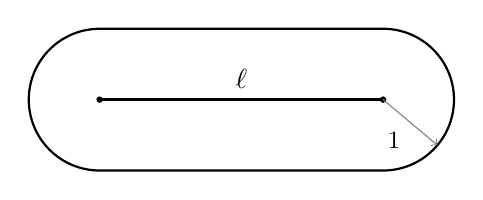
\begin{tikzpicture}[scale=0.9]
  \draw[thick] (0,1) -- (4,1) arc (90:-90:1) -- (0,-1) arc (270:90:1);
  \draw[very thick] (0,0) -- (4,0) node[midway,above] {$\ell$};
  \fill (0,0) circle (1.3pt) (4,0) circle (1.3pt);
  \draw[->,gray] (4,0) -- ++(-40:1) node[midway,below left,black] {\small$1$};
\end{tikzpicture}
\caption{An $\ell$-capsule: a segment of length $\ell$ plus a unit ball, drawn in a plane through the axis.}
\label{L3:fig:capsule}
\end{figure}

\begin{example}[$\ell$-capsules]\label{L3:ex:capsule}
Let $C=S_\ell+\Ball^d$, where $S_\ell$ is a segment of length $\ell$ \added{(the notes write ``$\ell\times\Ball^n$'')}.
\added{Then $r(C)=1$ and $C_1=S_\ell$. Take a radial gauge $F(\abs x)$ for $\Ball^d$ and $\gamma=1$, so $g(x)=F(d(x,S_\ell))$.
Write $I_k(F)=\int_{\R^k}F(\abs y)\,dy$. Points whose nearest point on $S_\ell$ is interior contribute a cylinder over $S_\ell$, and the two
ends together contribute a full ball's worth, so}
\[
  I(g)=\ell\cdot\frac{I_{d-1}(F)}{\vol(\Ball^{d-1})}\,\vol(\Ball^{d-1})+\frac{I_d(F)}{\vol(\Ball^d)}\,\vol(\Ball^d)
  =\ell\,I_{d-1}(F)+I_d(F),
\]
and
\[
  \vol(\ell\text{-capsule})=\ell\vol(\Ball^{d-1})+\vol(\Ball^d).
\]
Hence
\[
  \dens(\ell\text{-capsule})\le\frac{\ell\vol(\Ball^{d-1})+\vol(\Ball^d)}{\ell\,I_{d-1}(F)+I_d(F)}.
\]
\added{As $\ell\to\infty$ this tends to $\vol(\Ball^{d-1})/I_{d-1}(F)$, the $(d-1)$-dimensional ball bound for the same profile; for $d=3$ and
the improved $f$ above this is the value $.94$ from the table (assuming $f$ is a gauge in $\R^3$).}
\end{example}

\begin{remark}
\added{For a genuine cylinder $S_\ell\times\Ball^{d-1}$ (flat ends) the same computation works up to} end errors.
\end{remark}
